% Options for packages loaded elsewhere
\PassOptionsToPackage{unicode}{hyperref}
\PassOptionsToPackage{hyphens}{url}
\PassOptionsToPackage{dvipsnames,svgnames,x11names}{xcolor}
%
\documentclass[
  letterpaper,
  DIV=11,
  numbers=noendperiod]{scrartcl}

\usepackage{amsmath,amssymb}
\usepackage{iftex}
\ifPDFTeX
  \usepackage[T1]{fontenc}
  \usepackage[utf8]{inputenc}
  \usepackage{textcomp} % provide euro and other symbols
\else % if luatex or xetex
  \usepackage{unicode-math}
  \defaultfontfeatures{Scale=MatchLowercase}
  \defaultfontfeatures[\rmfamily]{Ligatures=TeX,Scale=1}
\fi
\usepackage{lmodern}
\ifPDFTeX\else  
    % xetex/luatex font selection
\fi
% Use upquote if available, for straight quotes in verbatim environments
\IfFileExists{upquote.sty}{\usepackage{upquote}}{}
\IfFileExists{microtype.sty}{% use microtype if available
  \usepackage[]{microtype}
  \UseMicrotypeSet[protrusion]{basicmath} % disable protrusion for tt fonts
}{}
\makeatletter
\@ifundefined{KOMAClassName}{% if non-KOMA class
  \IfFileExists{parskip.sty}{%
    \usepackage{parskip}
  }{% else
    \setlength{\parindent}{0pt}
    \setlength{\parskip}{6pt plus 2pt minus 1pt}}
}{% if KOMA class
  \KOMAoptions{parskip=half}}
\makeatother
\usepackage{xcolor}
\setlength{\emergencystretch}{3em} % prevent overfull lines
\setcounter{secnumdepth}{-\maxdimen} % remove section numbering
% Make \paragraph and \subparagraph free-standing
\ifx\paragraph\undefined\else
  \let\oldparagraph\paragraph
  \renewcommand{\paragraph}[1]{\oldparagraph{#1}\mbox{}}
\fi
\ifx\subparagraph\undefined\else
  \let\oldsubparagraph\subparagraph
  \renewcommand{\subparagraph}[1]{\oldsubparagraph{#1}\mbox{}}
\fi

\usepackage{color}
\usepackage{fancyvrb}
\newcommand{\VerbBar}{|}
\newcommand{\VERB}{\Verb[commandchars=\\\{\}]}
\DefineVerbatimEnvironment{Highlighting}{Verbatim}{commandchars=\\\{\}}
% Add ',fontsize=\small' for more characters per line
\usepackage{framed}
\definecolor{shadecolor}{RGB}{241,243,245}
\newenvironment{Shaded}{\begin{snugshade}}{\end{snugshade}}
\newcommand{\AlertTok}[1]{\textcolor[rgb]{0.68,0.00,0.00}{#1}}
\newcommand{\AnnotationTok}[1]{\textcolor[rgb]{0.37,0.37,0.37}{#1}}
\newcommand{\AttributeTok}[1]{\textcolor[rgb]{0.40,0.45,0.13}{#1}}
\newcommand{\BaseNTok}[1]{\textcolor[rgb]{0.68,0.00,0.00}{#1}}
\newcommand{\BuiltInTok}[1]{\textcolor[rgb]{0.00,0.23,0.31}{#1}}
\newcommand{\CharTok}[1]{\textcolor[rgb]{0.13,0.47,0.30}{#1}}
\newcommand{\CommentTok}[1]{\textcolor[rgb]{0.37,0.37,0.37}{#1}}
\newcommand{\CommentVarTok}[1]{\textcolor[rgb]{0.37,0.37,0.37}{\textit{#1}}}
\newcommand{\ConstantTok}[1]{\textcolor[rgb]{0.56,0.35,0.01}{#1}}
\newcommand{\ControlFlowTok}[1]{\textcolor[rgb]{0.00,0.23,0.31}{#1}}
\newcommand{\DataTypeTok}[1]{\textcolor[rgb]{0.68,0.00,0.00}{#1}}
\newcommand{\DecValTok}[1]{\textcolor[rgb]{0.68,0.00,0.00}{#1}}
\newcommand{\DocumentationTok}[1]{\textcolor[rgb]{0.37,0.37,0.37}{\textit{#1}}}
\newcommand{\ErrorTok}[1]{\textcolor[rgb]{0.68,0.00,0.00}{#1}}
\newcommand{\ExtensionTok}[1]{\textcolor[rgb]{0.00,0.23,0.31}{#1}}
\newcommand{\FloatTok}[1]{\textcolor[rgb]{0.68,0.00,0.00}{#1}}
\newcommand{\FunctionTok}[1]{\textcolor[rgb]{0.28,0.35,0.67}{#1}}
\newcommand{\ImportTok}[1]{\textcolor[rgb]{0.00,0.46,0.62}{#1}}
\newcommand{\InformationTok}[1]{\textcolor[rgb]{0.37,0.37,0.37}{#1}}
\newcommand{\KeywordTok}[1]{\textcolor[rgb]{0.00,0.23,0.31}{#1}}
\newcommand{\NormalTok}[1]{\textcolor[rgb]{0.00,0.23,0.31}{#1}}
\newcommand{\OperatorTok}[1]{\textcolor[rgb]{0.37,0.37,0.37}{#1}}
\newcommand{\OtherTok}[1]{\textcolor[rgb]{0.00,0.23,0.31}{#1}}
\newcommand{\PreprocessorTok}[1]{\textcolor[rgb]{0.68,0.00,0.00}{#1}}
\newcommand{\RegionMarkerTok}[1]{\textcolor[rgb]{0.00,0.23,0.31}{#1}}
\newcommand{\SpecialCharTok}[1]{\textcolor[rgb]{0.37,0.37,0.37}{#1}}
\newcommand{\SpecialStringTok}[1]{\textcolor[rgb]{0.13,0.47,0.30}{#1}}
\newcommand{\StringTok}[1]{\textcolor[rgb]{0.13,0.47,0.30}{#1}}
\newcommand{\VariableTok}[1]{\textcolor[rgb]{0.07,0.07,0.07}{#1}}
\newcommand{\VerbatimStringTok}[1]{\textcolor[rgb]{0.13,0.47,0.30}{#1}}
\newcommand{\WarningTok}[1]{\textcolor[rgb]{0.37,0.37,0.37}{\textit{#1}}}

\providecommand{\tightlist}{%
  \setlength{\itemsep}{0pt}\setlength{\parskip}{0pt}}\usepackage{longtable,booktabs,array}
\usepackage{calc} % for calculating minipage widths
% Correct order of tables after \paragraph or \subparagraph
\usepackage{etoolbox}
\makeatletter
\patchcmd\longtable{\par}{\if@noskipsec\mbox{}\fi\par}{}{}
\makeatother
% Allow footnotes in longtable head/foot
\IfFileExists{footnotehyper.sty}{\usepackage{footnotehyper}}{\usepackage{footnote}}
\makesavenoteenv{longtable}
\usepackage{graphicx}
\makeatletter
\def\maxwidth{\ifdim\Gin@nat@width>\linewidth\linewidth\else\Gin@nat@width\fi}
\def\maxheight{\ifdim\Gin@nat@height>\textheight\textheight\else\Gin@nat@height\fi}
\makeatother
% Scale images if necessary, so that they will not overflow the page
% margins by default, and it is still possible to overwrite the defaults
% using explicit options in \includegraphics[width, height, ...]{}
\setkeys{Gin}{width=\maxwidth,height=\maxheight,keepaspectratio}
% Set default figure placement to htbp
\makeatletter
\def\fps@figure{htbp}
\makeatother

\KOMAoption{captions}{tableheading}
\makeatletter
\@ifpackageloaded{caption}{}{\usepackage{caption}}
\AtBeginDocument{%
\ifdefined\contentsname
  \renewcommand*\contentsname{Table of contents}
\else
  \newcommand\contentsname{Table of contents}
\fi
\ifdefined\listfigurename
  \renewcommand*\listfigurename{List of Figures}
\else
  \newcommand\listfigurename{List of Figures}
\fi
\ifdefined\listtablename
  \renewcommand*\listtablename{List of Tables}
\else
  \newcommand\listtablename{List of Tables}
\fi
\ifdefined\figurename
  \renewcommand*\figurename{Figure}
\else
  \newcommand\figurename{Figure}
\fi
\ifdefined\tablename
  \renewcommand*\tablename{Table}
\else
  \newcommand\tablename{Table}
\fi
}
\@ifpackageloaded{float}{}{\usepackage{float}}
\floatstyle{ruled}
\@ifundefined{c@chapter}{\newfloat{codelisting}{h}{lop}}{\newfloat{codelisting}{h}{lop}[chapter]}
\floatname{codelisting}{Listing}
\newcommand*\listoflistings{\listof{codelisting}{List of Listings}}
\makeatother
\makeatletter
\makeatother
\makeatletter
\@ifpackageloaded{caption}{}{\usepackage{caption}}
\@ifpackageloaded{subcaption}{}{\usepackage{subcaption}}
\makeatother
\ifLuaTeX
  \usepackage{selnolig}  % disable illegal ligatures
\fi
\usepackage{bookmark}

\IfFileExists{xurl.sty}{\usepackage{xurl}}{} % add URL line breaks if available
\urlstyle{same} % disable monospaced font for URLs
\hypersetup{
  pdftitle={Social Sciences Intro to Statistics},
  colorlinks=true,
  linkcolor={blue},
  filecolor={Maroon},
  citecolor={Blue},
  urlcolor={Blue},
  pdfcreator={LaTeX via pandoc}}

\title{Social Sciences Intro to Statistics}
\usepackage{etoolbox}
\makeatletter
\providecommand{\subtitle}[1]{% add subtitle to \maketitle
  \apptocmd{\@title}{\par {\large #1 \par}}{}{}
}
\makeatother
\subtitle{Week 5.1 Inferential Statistics, about a single variable}
\author{}
\date{}

\begin{document}
\maketitle

Week 5: Learning goal - Formulate hypothesis testing both by hand and
with infer commands for a single population mean.

\section{Introduction}\label{introduction}

Lecture overview:

\begin{itemize}
\item
  Inferential statistics, about single variable
\item
  Hypothesis testing about a (single) population mean (by hand)
\end{itemize}

Load packages:

\begin{Shaded}
\begin{Highlighting}[]
\FunctionTok{library}\NormalTok{(tidyverse)}
\FunctionTok{library}\NormalTok{(ggplot2)}
\FunctionTok{library}\NormalTok{(labelled)}
\FunctionTok{library}\NormalTok{(patchwork)}

\CommentTok{\# Load ipeds dataset from course website}
\FunctionTok{load}\NormalTok{(}\FunctionTok{url}\NormalTok{(}\StringTok{\textquotesingle{}https://raw.githubusercontent.com/bcl96/Social{-}Sciences{-}Stats/main/data/ipeds/output\_data/panel\_data.RData\textquotesingle{}}\NormalTok{))}
\end{Highlighting}
\end{Shaded}

\begin{verbatim}
#> Rows: 965
#> Columns: 38
#> $ instnm            <chr> "Alabama A & M University", "University of Alabama a~
#> $ unitid            <dbl> 100654, 100663, 100706, 100724, 100751, 100830, 1008~
#> $ opeid6            <chr> "001002", "001052", "001055", "001005", "001051", "0~
#> $ opeid             <chr> "00100200", "00105200", "00105500", "00100500", "001~
#> $ control           <dbl+lbl> 1, 1, 1, 1, 1, 1, 1, 2, 1, 1, 1, 1, 2, 1, 1, 2, ~
#> $ c15basic          <dbl+lbl> 18, 15, 16, 19, 16, 18, 16, 20, 18, 18, 19, 18, ~
#> $ stabbr            <chr+lbl> "AL", "AL", "AL", "AL", "AL", "AL", "AL", "AL", ~
#> $ city              <chr> "Normal", "Birmingham", "Huntsville", "Montgomery", ~
#> $ zip               <chr> "35762", "35294-0110", "35899", "36104-0271", "35487~
#> $ locale            <dbl+lbl> 12, 12, 12, 12, 13, 12, 13, 12, 23, 43, 21, 13, ~
#> $ region            <dbl+lbl> 5, 5, 5, 5, 5, 5, 5, 5, 5, 5, 5, 5, 5, 5, 5, 5, ~
#> $ tuit_grad_res     <dbl> 10128, 8424, 10632, 7416, 11100, 7812, 10386, 15325,~
#> $ fee_grad_res      <dbl> 1414, 0, 1054, 2740, 690, 766, 1784, 900, 1000, 190,~
#> $ tuit_grad_nres    <dbl> 20160, 19962, 24430, 14832, 31460, 17550, 31158, 153~
#> $ fee_grad_nres     <dbl> 1414, 0, 1054, 2740, 690, 766, 1784, 900, 1000, 190,~
#> $ tuit_md_res       <dbl> NA, 31198, NA, NA, 31198, NA, NA, NA, NA, NA, NA, NA~
#> $ fee_md_res        <dbl> NA, 3464, NA, NA, 0, NA, NA, NA, NA, NA, NA, NA, NA,~
#> $ tuit_md_nres      <dbl> NA, 62714, NA, NA, 62714, NA, NA, NA, NA, NA, NA, NA~
#> $ fee_md_nres       <dbl> NA, 3464, NA, NA, 0, NA, NA, NA, NA, NA, NA, NA, NA,~
#> $ tuit_law_res      <dbl> NA, NA, NA, NA, 24080, NA, NA, 39000, NA, NA, NA, NA~
#> $ fee_law_res       <dbl> NA, NA, NA, NA, 300, NA, NA, 325, NA, NA, NA, NA, 65~
#> $ tuit_law_nres     <dbl> NA, NA, NA, NA, 44470, NA, NA, 39000, NA, NA, NA, NA~
#> $ fee_law_nres      <dbl> NA, NA, NA, NA, 300, NA, NA, 325, NA, NA, NA, NA, 65~
#> $ books_supplies    <dbl> 1600, 1200, 2416, 1600, 800, 1200, 1200, 1800, 998, ~
#> $ roomboard_off     <dbl> 9520, 14330, 11122, 7320, 14426, 10485, 14998, 8020,~
#> $ oth_expense_off   <dbl> 3090, 6007, 4462, 5130, 4858, 4030, 6028, 4600, 3318~
#> $ tuitfee_grad_res  <dbl> 11542, 8424, 11686, 10156, 11790, 8578, 12170, 16225~
#> $ tuitfee_grad_nres <dbl> 21574, 19962, 25484, 17572, 32150, 18316, 32942, 162~
#> $ tuitfee_md_res    <dbl> NA, 34662, NA, NA, 31198, NA, NA, NA, NA, NA, NA, NA~
#> $ tuitfee_md_nres   <dbl> NA, 66178, NA, NA, 62714, NA, NA, NA, NA, NA, NA, NA~
#> $ tuitfee_law_res   <dbl> NA, NA, NA, NA, 24380, NA, NA, 39325, NA, NA, NA, NA~
#> $ tuitfee_law_nres  <dbl> NA, NA, NA, NA, 44770, NA, NA, 39325, NA, NA, NA, NA~
#> $ coa_grad_res      <dbl> 25752, 29961, 29686, 24206, 31874, 24293, 34396, 306~
#> $ coa_grad_nres     <dbl> 35784, 41499, 43484, 31622, 52234, 34031, 55168, 306~
#> $ coa_md_res        <dbl> NA, 56199, NA, NA, 51282, NA, NA, NA, NA, NA, NA, NA~
#> $ coa_md_nres       <dbl> NA, 87715, NA, NA, 82798, NA, NA, NA, NA, NA, NA, NA~
#> $ coa_law_res       <dbl> NA, NA, NA, NA, 44464, NA, NA, 53745, NA, NA, NA, NA~
#> $ coa_law_nres      <dbl> NA, NA, NA, NA, 64854, NA, NA, 53745, NA, NA, NA, NA~
#> Rows: 200
#> Columns: 4
#> $ norm_dist    <dbl> 42.70513, 50.24400, 61.29008, 45.47494, 44.74406, 47.9912~
#> $ rskew_dist   <dbl> 0.34451771, 0.31359906, 0.09375337, 0.05581678, 0.0744584~
#> $ lskew_dist   <dbl> 0.6554823, 0.6864009, 0.9062466, 0.9441832, 0.9255415, 0.~
#> $ stdnorm_dist <dbl> -1.45897348, 0.04880097, 2.25801577, -0.90501164, -1.0511~
#> [1] 32528.35
#> [1] 31620.8
\end{verbatim}

\section{Fundamentals of inferential
statistics}\label{fundamentals-of-inferential-statistics}

Inferential statistics is a method to use quantitative data to answer
questions we may have about a population that we are observing.
Fundamentals of inferential statistics include:

\begin{itemize}
\item
  Hypothesis testing: This is also known as the test of significance,
  used by testing claims about populations by weighing quantitative
  evidence for or against a conclusion.
\item
  Confidence intervals: This method uses samples from targeted
  populations to estimate the true value of a parameter as a range of
  values.
\item
  Regression Analysis: This method finds trends in data and predict
  future values of a time series.
\item
  Correlation: This is a statistical test used to determine if there is
  a statistically significant relationship between two variables.
\item
  T-test: This method compares the values of two groups in order to
  determine if there is a significant difference between two data sets
  from the same population.
\item
  ANOVA: This test is used to make inferences about population means for
  any number of groups and independent variables.
\item
  Chi-squared test: This test is used to help draw conclusions about a
  population based on a sample, such as whether two variables are
  related in the population.
\end{itemize}

As you continue on learning about statistics, you will encounter the
rest of these methods. Today we are going to start with hypothesis
testing about a single population mean.

\section{Hypothesis testing about a (single) population
mean}\label{hypothesis-testing-about-a-single-population-mean}

\subsection{What and Why hypothesis
testing}\label{what-and-why-hypothesis-testing}

Quantitative research in social sciences often proceeds as follows:

\begin{itemize}
\tightlist
\item
  Develop a research question (which guides our research)
\item
  Develop one (or more) testable hypothesis based on that research
  question
\item
  Obtain data necessary to test the hypothesis
\item
  Test the hypothesis by applying an appropriate statistical test to the
  data
\end{itemize}

Some examples of research questions co-authors and I have answered over
the years:

\begin{itemize}
\tightlist
\item
  What is the relationship between state appropriations and nonresident
  enrollment at public universities {[}@RN3753{]}?
\item
  What is the effect of nonresident enrollment growth on the number of
  resident students enrolled at public research universities
  {[}@RN4290{]}?
\item
  What is the effect of participation in the Mexican American Studies
  program on the probability of high school graduation for students in
  the Tucscon Unified School District {[}@RN3292{]}?
\item
  Are high schools with a higher percentage of white students more
  likely to receive recruiting visits from university admissions officer
  than high schools with a lower percentage of white students
  {[}@RN4450{]}?
\end{itemize}

For each of these journal articles, we answered the research question by
developing a ``testable hypothesis'' and testing that hypothesis using
some statistical test

Developing testable hypothesis is central to univariate statistical
analysis (one variable), bivariate statistical analysis (two variables),
and multivariate statistical analysis (3+ variables, usually a
regression model)

Example hypotheses for univariate, bivariate, multivariate statistical
analyses

\begin{itemize}
\tightlist
\item
  Univariate statistics (hypothesis tests about a single population
  mean)

  \begin{itemize}
  \tightlist
  \item
    Hypothesis: the average annual cost of attendance for graduate
    school (tuition + fees + living expenses) is \$50,000
  \end{itemize}
\item
  Bivariate statistics {[}hypothesis tests about comparing two
  population means{]}

  \begin{itemize}
  \tightlist
  \item
    Hypothesis: the average annual cost of attendance for graduate
    school (tuition + fees + living expenses) at private universities is
    higher than public universities
  \item
    Hypothesis: the average annual cost of attendance for graduate
    school (tuition + fees + living expenses) at universities in urban
    areas is higher than universities in suburban areas
  \end{itemize}
\item
  Multivariate statistics (usually a regression model with one dependent
  variable, one independent variable of interest, and one or more
  ``control'' variables)

  \begin{itemize}
  \tightlist
  \item
    where dependent variable (Y) = cost of attendance; independent
    variable of interest (X) = private or public university; control
    variable = level of urbanization
  \item
    Hypothesis: cost of attendance for graduate school is higher at
    private universities than public universities, even after
    controlling for level of urbanization
  \end{itemize}
\end{itemize}

Why learn how to do hypothesis testing about a single population mean
when this class is supposed to be about regression (and hypothesis tests
about regression models)?

\begin{itemize}
\tightlist
\item
  You must learn the general principles/concepts about using
  point-estimates from sample data to test hypotheses about population
  parameters
\item
  The simplest practical application of these general
  principles/concepts is testing hypotheses about the value of a single
  population mean
\item
  The concepts/steps for hypotheses tests about a single population mean
  are exactly the same as those for testing hypotheses about regression
  models
\end{itemize}

\subsection{Overview of steps in hypothesis
testing}\label{overview-of-steps-in-hypothesis-testing}

These are the general steps in hypothesis testing:

\begin{enumerate}
\def\labelenumi{\arabic{enumi}.}
\tightlist
\item
  \textbf{Hypothesis}

  \begin{itemize}
  \tightlist
  \item
    formally state your ``null'' and ``alternative'' hypothesis
  \end{itemize}
\item
  \textbf{Assumptions}

  \begin{itemize}
  \tightlist
  \item
    state assumptions that are relied upon by the statistical test you
    are using to test your hypothesis
  \end{itemize}
\item
  \textbf{Test statistic}

  \begin{itemize}
  \tightlist
  \item
    Using some appropriate statistical analysis, calculate the ``test
    statistic'' necessary to test your hypothesis
  \end{itemize}
\item
  \textbf{p-value (means probability value)}

  \begin{itemize}
  \tightlist
  \item
    calculate the probability of observing a test statistic as large or
    larger as the one you calculated
  \end{itemize}
\item
  \textbf{Alpha level/rejection region and conclusion}

  \begin{itemize}
  \tightlist
  \item
    decide on the ``alpha level,'' the p-value associated with rejection
    of the null hypothesis
  \item
    compare the p-value you you observed to the alpha level and make a
    conclusion about your hypothesis test
  \end{itemize}
\end{enumerate}

In real research projects, do researchers always follow these exact
steps? In this exact order?

\begin{itemize}
\tightlist
\item
  Yes, they follow these steps
\item
  But researchers do not necessarily follow steps in this exact order

  \begin{itemize}
  \tightlist
  \item
    e.g., usually, you would decide on an ``alpha level'' (rejection
    region) prior to conducting the statistical analysis
  \end{itemize}
\item
  Often, researchers will not write out each step as formally as we will
  ask you all to do.

  \begin{itemize}
  \tightlist
  \item
    We ask you to write out each step to give you practice. Later in the
    quarter, you won't have to write out each step
  \end{itemize}
\end{itemize}

Example we will use to introduce steps in hypothesis testing

\begin{itemize}
\tightlist
\item
  The population mean cost of attendance (COA) for full-time (resident)
  graduate students, \(\mu_Y\), is \texttt{\$28,000}
\end{itemize}

How we will teach you the steps in hypothesis testing in this lecture

\begin{itemize}
\tightlist
\item
  First, Introduce individual steps in detail, so that you develop a
  deep, conceptual understanding of each step

  \begin{itemize}
  \tightlist
  \item
    But when thinking about an individual step in detail, it can be hard
    to remember its relationship to other steps and to hypothesis
    testing as a whole
  \end{itemize}
\item
  Second, we will do another pratical example, where we work through all
  steps more quickly

  \begin{itemize}
  \tightlist
  \item
    so you can get a better sense of the hypothesis testing process as a
    whole and the relationships between steps
  \end{itemize}
\end{itemize}

\subsection{Hypotheses}\label{hypotheses}

This section presents a more formal introduction to hypotheses, focusing
on univariate statistical analyses rather than bivariate or multivariate

Recall that the goal of inferential statistics is to make statements
about a population of interest based on data from a representative
sample from the population.

\begin{itemize}
\tightlist
\item
  We make a hypotheses about a population parameter (e.g., population
  mean of variable \(Y\) denotes \(\mu_Y\))
\item
  Knowing the true value of the population parameter would require
  having data on all observations in the population
\item
  Usually, we do not have data on the entire population
\item
  We use sample data to test hypotheses about the population
\end{itemize}

Definition

\begin{itemize}
\tightlist
\item
  In statistics, a \textbf{hypothesis} is a declarative statement about
  a population.
\end{itemize}

In univariate statistical analyses, we make a hypothesis about one
population paramaeter (e.g., population mean \(\mu_Y\)) from one
population of interest (e.g., all ``research'' universities and
``master's'' universities, as defined by the Carnegie Classification)

\begin{Shaded}
\begin{Highlighting}[]
\NormalTok{df\_ipeds\_pop }\SpecialCharTok{\%\textgreater{}\%} \FunctionTok{glimpse}\NormalTok{()}
\CommentTok{\#\textgreater{} Rows: 965}
\CommentTok{\#\textgreater{} Columns: 38}
\CommentTok{\#\textgreater{} $ instnm            \textless{}chr\textgreater{} "Alabama A \& M University", "University of Alabama a\textasciitilde{}}
\CommentTok{\#\textgreater{} $ unitid            \textless{}dbl\textgreater{} 100654, 100663, 100706, 100724, 100751, 100830, 1008\textasciitilde{}}
\CommentTok{\#\textgreater{} $ opeid6            \textless{}chr\textgreater{} "001002", "001052", "001055", "001005", "001051", "0\textasciitilde{}}
\CommentTok{\#\textgreater{} $ opeid             \textless{}chr\textgreater{} "00100200", "00105200", "00105500", "00100500", "001\textasciitilde{}}
\CommentTok{\#\textgreater{} $ control           \textless{}dbl+lbl\textgreater{} 1, 1, 1, 1, 1, 1, 1, 2, 1, 1, 1, 1, 2, 1, 1, 2, \textasciitilde{}}
\CommentTok{\#\textgreater{} $ c15basic          \textless{}dbl+lbl\textgreater{} 18, 15, 16, 19, 16, 18, 16, 20, 18, 18, 19, 18, \textasciitilde{}}
\CommentTok{\#\textgreater{} $ stabbr            \textless{}chr+lbl\textgreater{} "AL", "AL", "AL", "AL", "AL", "AL", "AL", "AL", \textasciitilde{}}
\CommentTok{\#\textgreater{} $ city              \textless{}chr\textgreater{} "Normal", "Birmingham", "Huntsville", "Montgomery", \textasciitilde{}}
\CommentTok{\#\textgreater{} $ zip               \textless{}chr\textgreater{} "35762", "35294{-}0110", "35899", "36104{-}0271", "35487\textasciitilde{}}
\CommentTok{\#\textgreater{} $ locale            \textless{}dbl+lbl\textgreater{} 12, 12, 12, 12, 13, 12, 13, 12, 23, 43, 21, 13, \textasciitilde{}}
\CommentTok{\#\textgreater{} $ region            \textless{}dbl+lbl\textgreater{} 5, 5, 5, 5, 5, 5, 5, 5, 5, 5, 5, 5, 5, 5, 5, 5, \textasciitilde{}}
\CommentTok{\#\textgreater{} $ tuit\_grad\_res     \textless{}dbl\textgreater{} 10128, 8424, 10632, 7416, 11100, 7812, 10386, 15325,\textasciitilde{}}
\CommentTok{\#\textgreater{} $ fee\_grad\_res      \textless{}dbl\textgreater{} 1414, 0, 1054, 2740, 690, 766, 1784, 900, 1000, 190,\textasciitilde{}}
\CommentTok{\#\textgreater{} $ tuit\_grad\_nres    \textless{}dbl\textgreater{} 20160, 19962, 24430, 14832, 31460, 17550, 31158, 153\textasciitilde{}}
\CommentTok{\#\textgreater{} $ fee\_grad\_nres     \textless{}dbl\textgreater{} 1414, 0, 1054, 2740, 690, 766, 1784, 900, 1000, 190,\textasciitilde{}}
\CommentTok{\#\textgreater{} $ tuit\_md\_res       \textless{}dbl\textgreater{} NA, 31198, NA, NA, 31198, NA, NA, NA, NA, NA, NA, NA\textasciitilde{}}
\CommentTok{\#\textgreater{} $ fee\_md\_res        \textless{}dbl\textgreater{} NA, 3464, NA, NA, 0, NA, NA, NA, NA, NA, NA, NA, NA,\textasciitilde{}}
\CommentTok{\#\textgreater{} $ tuit\_md\_nres      \textless{}dbl\textgreater{} NA, 62714, NA, NA, 62714, NA, NA, NA, NA, NA, NA, NA\textasciitilde{}}
\CommentTok{\#\textgreater{} $ fee\_md\_nres       \textless{}dbl\textgreater{} NA, 3464, NA, NA, 0, NA, NA, NA, NA, NA, NA, NA, NA,\textasciitilde{}}
\CommentTok{\#\textgreater{} $ tuit\_law\_res      \textless{}dbl\textgreater{} NA, NA, NA, NA, 24080, NA, NA, 39000, NA, NA, NA, NA\textasciitilde{}}
\CommentTok{\#\textgreater{} $ fee\_law\_res       \textless{}dbl\textgreater{} NA, NA, NA, NA, 300, NA, NA, 325, NA, NA, NA, NA, 65\textasciitilde{}}
\CommentTok{\#\textgreater{} $ tuit\_law\_nres     \textless{}dbl\textgreater{} NA, NA, NA, NA, 44470, NA, NA, 39000, NA, NA, NA, NA\textasciitilde{}}
\CommentTok{\#\textgreater{} $ fee\_law\_nres      \textless{}dbl\textgreater{} NA, NA, NA, NA, 300, NA, NA, 325, NA, NA, NA, NA, 65\textasciitilde{}}
\CommentTok{\#\textgreater{} $ books\_supplies    \textless{}dbl\textgreater{} 1600, 1200, 2416, 1600, 800, 1200, 1200, 1800, 998, \textasciitilde{}}
\CommentTok{\#\textgreater{} $ roomboard\_off     \textless{}dbl\textgreater{} 9520, 14330, 11122, 7320, 14426, 10485, 14998, 8020,\textasciitilde{}}
\CommentTok{\#\textgreater{} $ oth\_expense\_off   \textless{}dbl\textgreater{} 3090, 6007, 4462, 5130, 4858, 4030, 6028, 4600, 3318\textasciitilde{}}
\CommentTok{\#\textgreater{} $ tuitfee\_grad\_res  \textless{}dbl\textgreater{} 11542, 8424, 11686, 10156, 11790, 8578, 12170, 16225\textasciitilde{}}
\CommentTok{\#\textgreater{} $ tuitfee\_grad\_nres \textless{}dbl\textgreater{} 21574, 19962, 25484, 17572, 32150, 18316, 32942, 162\textasciitilde{}}
\CommentTok{\#\textgreater{} $ tuitfee\_md\_res    \textless{}dbl\textgreater{} NA, 34662, NA, NA, 31198, NA, NA, NA, NA, NA, NA, NA\textasciitilde{}}
\CommentTok{\#\textgreater{} $ tuitfee\_md\_nres   \textless{}dbl\textgreater{} NA, 66178, NA, NA, 62714, NA, NA, NA, NA, NA, NA, NA\textasciitilde{}}
\CommentTok{\#\textgreater{} $ tuitfee\_law\_res   \textless{}dbl\textgreater{} NA, NA, NA, NA, 24380, NA, NA, 39325, NA, NA, NA, NA\textasciitilde{}}
\CommentTok{\#\textgreater{} $ tuitfee\_law\_nres  \textless{}dbl\textgreater{} NA, NA, NA, NA, 44770, NA, NA, 39325, NA, NA, NA, NA\textasciitilde{}}
\CommentTok{\#\textgreater{} $ coa\_grad\_res      \textless{}dbl\textgreater{} 25752, 29961, 29686, 24206, 31874, 24293, 34396, 306\textasciitilde{}}
\CommentTok{\#\textgreater{} $ coa\_grad\_nres     \textless{}dbl\textgreater{} 35784, 41499, 43484, 31622, 52234, 34031, 55168, 306\textasciitilde{}}
\CommentTok{\#\textgreater{} $ coa\_md\_res        \textless{}dbl\textgreater{} NA, 56199, NA, NA, 51282, NA, NA, NA, NA, NA, NA, NA\textasciitilde{}}
\CommentTok{\#\textgreater{} $ coa\_md\_nres       \textless{}dbl\textgreater{} NA, 87715, NA, NA, 82798, NA, NA, NA, NA, NA, NA, NA\textasciitilde{}}
\CommentTok{\#\textgreater{} $ coa\_law\_res       \textless{}dbl\textgreater{} NA, NA, NA, NA, 44464, NA, NA, 53745, NA, NA, NA, NA\textasciitilde{}}
\CommentTok{\#\textgreater{} $ coa\_law\_nres      \textless{}dbl\textgreater{} NA, NA, NA, NA, 64854, NA, NA, 53745, NA, NA, NA, NA\textasciitilde{}}

\FunctionTok{mean}\NormalTok{(df\_ipeds\_pop}\SpecialCharTok{$}\NormalTok{coa\_grad\_res, }\AttributeTok{na.rm =} \ConstantTok{TRUE}\NormalTok{)}
\CommentTok{\#\textgreater{} [1] 32528.35}
\end{Highlighting}
\end{Shaded}

\subsubsection{Null and Alternative
hypothesis}\label{null-and-alternative-hypothesis}

When developing a hypothesis for quantitative research, we always
specify a \textbf{null hypothesis (\(H_0\))} AND an \textbf{alternative
hypothesis (\(H_a\))}

\textbf{Null hypothesis (\(H_0\))}

\begin{itemize}
\tightlist
\item
  In univariate statistics, a null hypothesis (\(H_0\)) is a declarative
  statement that the population parameter has a specific value
\item
  (in words) \(H_0:\) the population mean cost of attendance for for
  full-time (resident) graduate students, \(\mu_Y\), is
  \texttt{\$28,000}
\item
  (using symbols) \(H_0:\mu_Y = \mu_{Y0} = \$28,000\)

  \begin{itemize}
  \tightlist
  \item
    where \(\mu_{Y0}\) refers to the parameter value associated with the
    null hypothesis
  \item
    when testing a hypothesis about a single population mean, we can
    refer to \(\mu_{Y0}\) as the ``null population mean''
  \end{itemize}
\end{itemize}

\textbf{Alternative hypothesis (\(H_a\))}

\begin{itemize}
\tightlist
\item
  An alternative hypothesis (\(H_a\)) is a declarative statement that
  the population parameter falls in some alternative range of values as
  compared to the value declared by the null hypothesis
\item
  There are two kinds of alternative hypotheses: two-sided; and
  one-sided
\item
  for a given null hypothesis (\(H_0\)), there will always be one
  two-sided alternative hypothesis and two different one-sided
  hypotheses
\end{itemize}

Two-sided alternative hypothesis

\begin{itemize}
\tightlist
\item
  (in words) \(H_a:\) the population mean mean cost of attendance for
  for full-time (resident) graduate students, \(\mu_Y\), is not equal to
  \texttt{\$28,000}
\item
  (using symbols) \(H_a:\mu_Y \neq \$28,000\)
\end{itemize}

One-sided alternative hypothesis (mean is greater than \(\$28,000\))

\begin{itemize}
\tightlist
\item
  (in words) \(H_a:\) the population mean mean cost of attendance for
  for full-time (resident) graduate students, \(\mu_Y\), is greater than
  \texttt{\$28,000}
\item
  (using symbols) \(H_a:\mu_Y > \$28,000\)
\end{itemize}

One-sided alternative hypothesis (mean is less than \(\$28,000\))

\begin{itemize}
\tightlist
\item
  (in words) \(H_a:\) the population mean mean cost of attendance for
  for full-time (resident) graduate students, \(\mu_Y\), is less than
  \texttt{\$28,000}
\item
  (using symbols) \(H_a:\mu_Y < \$28,000\)
\end{itemize}

\textbf{Example of null and alternative hypotheses for bivariate
statistical analysis}

Research question:

\begin{itemize}
\tightlist
\item
  Is the population mean annual cost of attendance for graduate school
  at public universities (\(\mu_{Y_{{pub}}}\)) different from the
  population mean annual cost of attendance for graduate school at
  private universities (\(\mu_{Y_{{priv}}}\))?
\end{itemize}

Null and alternative hypotheses

\begin{itemize}
\tightlist
\item
  null hypothesis (\(H_0\))

  \begin{itemize}
  \tightlist
  \item
    (in words): \(H_0:\) the population mean annual cost of attendance
    for graduate school at public universities (\(\mu_{Y_{{pub}}}\)) is
    the same as the population mean annual cost of attendance for
    graduate school at private universities (\(\mu_{Y_{{priv}}}\))
  \item
    (symbols): \(H_0: \mu_{Y_{{pub}}} = \mu_{Y_{{priv}}}\)
  \end{itemize}
\item
  Two-sided alternative hypothesis

  \begin{itemize}
  \tightlist
  \item
    (in words): \(H_a:\) the population mean annual cost of attendance
    for graduate school at public universities (\(\mu_{Y_{{pub}}}\)) is
    different than the population mean annual cost of attendance for
    graduate school at private universities (\(\mu_{Y_{{priv}}}\))
  \item
    (symbols): \(H_a: \mu_{Y_{{pub}}} \neq \mu_{Y_{{priv}}}\)
  \end{itemize}
\item
  One-sided alternative hypothesis (\(pub < priv\))

  \begin{itemize}
  \tightlist
  \item
    (in words): \(H_a:\) the population mean annual cost of attendance
    for graduate school at public universities (\(\mu_{Y_{{pub}}}\)) is
    less than than the population mean annual cost of attendance for
    graduate school at private universities (\(\mu_{Y_{{priv}}}\))
  \item
    (symbols): \(H_a: \mu_{Y_{{pub}}} < \mu_{Y_{{priv}}}\)
  \item
    note: this is the same as a one-sided hypothesis where we
    hypothesize \(priv > pub\)
  \end{itemize}
\item
  One-sided alternative hypothesis (\$pub \textgreater{} priv \$)

  \begin{itemize}
  \tightlist
  \item
    (in words): \(H_a:\) the population mean annual cost of attendance
    for graduate school at public universities (\(\mu_{Y_{{pub}}}\)) is
    greater than than the population mean annual cost of attendance for
    graduate school at private universities (\(\mu_{Y_{{priv}}}\))
  \item
    (symbols): \(H_a: \mu_{Y_{{pub}}} > \mu_{Y_{{priv}}}\)
  \item
    note: this is the same as a one-sided hypothesis where we
    hypothesize \(priv < pub\)
  \end{itemize}
\end{itemize}

\subsubsection{Two-sided or one-sided alternative
hypotheses?}\label{two-sided-or-one-sided-alternative-hypotheses}

In real research projects, we are not usually testing a hypothesis about
a single population mean (univariate analysis). Rather, we are usually
comparing population means of two different groups (bivariate analysis)
or we are examining the relationship between an independent variable and
the dependent variable after controlling for other variables
(multivariate regression analysis)

Prior to conducting analyses, we usually have an expectation/suspicion
about the result

\begin{itemize}
\tightlist
\item
  For most bivariate analyses, we usually suspect that one particular
  group is has a higher mean value than the other

  \begin{itemize}
  \tightlist
  \item
    e.g., we suspect that mean cost of attendance at private
    universities
  \item
    this suggests a one-sided alternative hypothesis \(H_a\)
  \end{itemize}
\item
  For most multivariate analyses, we usually suspect the direction of
  the relationship between \(X\) and \(Y\)

  \begin{itemize}
  \tightlist
  \item
    e.g., we expect that ``hours spent studying'' (\(X\)) has a positive
    relationship with ``grade point average'' (\(Y\)) rather than
    thinking ``the relationship between hours spent studying (\(X\)) and
    grad point average (\(Y\)) does not equal zero
  \item
    this suggests a one-sided alternative hypothesis \(H_a\)
  \end{itemize}
\end{itemize}

Should we specify two-sided or one-sided alternative hypothesis,
\(H_a\)?

\begin{itemize}
\tightlist
\item
  For univariate and bivariate statistical analyses, researchers specify
  a two-sided alternative hypothesis more often than a one-sided
  alternative alternative hypothesis

  \begin{itemize}
  \tightlist
  \item
    often, researchers specify a two-sided alternative hypothesis even
    when they strongly believe one particular group has a larger
    population mean then the other
  \end{itemize}
\item
  For multivariate regression analyses, researchers \textbf{always}
  specify and test two-sided alternative hypotheses

  \begin{itemize}
  \tightlist
  \item
    even when they strongly believe the relationship between \(X\) and
    \(Y\) is positive; and even when they strongly believe the
    relationship between \(X\) and \(Y\) is positive
  \end{itemize}
\item
  Why this preference for two-sided alternative hypotheses in real
  research projects?

  \begin{itemize}
  \tightlist
  \item
    two-sided alternative hypotheses are more ``conservative'' than
    one-sided alternative hypotheses;
  \item
    that is, if you specify a two-sided alternative hypothesis, \(H_a\),
    and reject the null hypothesis, \(H_0\), then it is necessarily true
    that we would have rejected then null hypothesis, \(H_0\), had we
    specified a one-sided alternative hypothesis, \(H_a\)
  \end{itemize}
\end{itemize}

\subsection{Test statistic}\label{test-statistic}

restate null, \(H_0\), and alternative (two-sided), \(H_a\), hypothesis
for our practical example

\begin{itemize}
\tightlist
\item
  \(H_0\)

  \begin{itemize}
  \tightlist
  \item
    (in words) \(H_0:\) the population mean cost of attendance for for
    full-time (resident) graduate students, \(\mu_Y\), is \$28,000
  \item
    (symbols) \(H_0: \mu_Y = \mu_{Y0} = \$28,000\)
  \end{itemize}
\item
  \(H_a\)

  \begin{itemize}
  \tightlist
  \item
    (in words) \(H_a:\) the population mean mean cost of attendance for
    for full-time (resident) graduate students, \(\mu_Y\), is not equal
    to \$28,000
  \item
    (symbols) \(H_a: \mu_Y \ne \$28,000\)
  \end{itemize}
\end{itemize}

We must conduct a formal statistical test to decide whether we should
reject the null hypothesis

\begin{itemize}
\tightlist
\item
  this is true for testing hypotheses about a population mean from a
  single population; testing hypotheses about whether two population
  means are equal; testing hypotheses about a regression coefficient,
  etc.
\item
  \textbf{key to understanding hypothesis testing}: We conduct our test
  under the assumption that the null hypothesis, \(H_0\), is true
\end{itemize}

Logic of the test statistic

\begin{itemize}
\tightlist
\item
  What the test statistic calculates

  \begin{itemize}
  \tightlist
  \item
    if the null hypothesis is true, how unlikely would it be to randomly
    draw the sample estimate (e.g., sample mean \(\bar{Y}\)) at least as
    far away from the null hypothesis value as the one we observed in
    our single random sample
  \item
    e.g., ``if the null hypothesis is true, there is a 1.5\% chance of
    observing a sample mean at least as far away from the null
    hypothesis value (\(\mu_{Y0} = \$28,000\)) as the one we observed in
    our single random sample
  \end{itemize}
\item
  Logic of the test statistic

  \begin{itemize}
  \tightlist
  \item
    if -- under the assumption that the null hypothesis is true -- it
    would be very unlikely to observe the sample estimate we observed,
    then it is unlikely that the null hypothesis is true
  \end{itemize}
\end{itemize}

\textbf{General formula for test statistic (for pretty much any kind of
hypothesis test)}:

\[ test\_statistic = \frac{sample\_estimate - value\_associated\_with\_H_0}{sample\_standard\_error}\]
\textbf{Formula for test statistic about a single population mean}

\begin{itemize}
\tightlist
\item
  in words:

  \begin{itemize}
  \tightlist
  \item
    test-statistic \(t\) equals difference between the sample mean
    \(\bar{Y}\) and the population mean associated with the null
    hypothesis \(\mu_{Y0}\) divided by the sample standard error of the
    sample mean \(\hat{\sigma}_{\bar{Y}}\)
  \end{itemize}
\item
  equation:

  \begin{itemize}
  \tightlist
  \item
    \(t = \frac{\bar{Y} - \mu_{Y0}}{\hat{\sigma}_{\bar{Y}}}\)
  \end{itemize}
\item
  where:

  \begin{itemize}
  \tightlist
  \item
    \(\hat{\sigma}_{Y}\) refers to sample standard deviation of variable
    \(Y\)
  \item
    \(n\) refers to sample size
  \item
    sample standard error of the sample mean
    \(= \hat{\sigma}_{\bar{Y}} = \frac{\hat{\sigma}_{Y}}{\sqrt{n}}\)
  \end{itemize}
\end{itemize}

\textbf{Calculating t-test statistic for our practical example}

\(H_0: \mu_Y = \mu_{Y0} = \$28,000\) ; \(H_a: \mu_Y \ne \$28,000\)

Calculate components of t-test (using functions and by hand)

\begin{Shaded}
\begin{Highlighting}[]
\CommentTok{\# sample size}
  \FunctionTok{length}\NormalTok{(df\_ipeds\_sample}\SpecialCharTok{$}\NormalTok{coa\_grad\_res) }\CommentTok{\# assuming no missing observations}
\CommentTok{\#\textgreater{} [1] 200}
\NormalTok{  df\_ipeds\_sample }\SpecialCharTok{\%\textgreater{}\%} \FunctionTok{summarize}\NormalTok{(}\AttributeTok{n\_non\_miss =} \FunctionTok{sum}\NormalTok{(}\SpecialCharTok{!}\NormalTok{(}\FunctionTok{is.na}\NormalTok{(coa\_grad\_res)))) }\CommentTok{\# count only number of non{-}missing}
\CommentTok{\#\textgreater{} \# A tibble: 1 x 1}
\CommentTok{\#\textgreater{}   n\_non\_miss}
\CommentTok{\#\textgreater{}        \textless{}int\textgreater{}}
\CommentTok{\#\textgreater{} 1        200}

\CommentTok{\# sample mean of coa\_grad\_res}
  \FunctionTok{mean}\NormalTok{(df\_ipeds\_sample}\SpecialCharTok{$}\NormalTok{coa\_grad\_res, }\AttributeTok{na.rm =} \ConstantTok{TRUE}\NormalTok{) }\CommentTok{\# using function}
\CommentTok{\#\textgreater{} [1] 31620.8}
  
\CommentTok{\# sample standard deviation of coa\_grad\_res}
  \FunctionTok{sd}\NormalTok{(df\_ipeds\_sample}\SpecialCharTok{$}\NormalTok{coa\_grad\_res, }\AttributeTok{na.rm =} \ConstantTok{TRUE}\NormalTok{)}
\CommentTok{\#\textgreater{} [1] 11298.37}

\CommentTok{\# sample standard error of sample mean of coa\_grad\_res = std\_dev/sqrt(n)}
  \FunctionTok{sd}\NormalTok{(df\_ipeds\_sample}\SpecialCharTok{$}\NormalTok{coa\_grad\_res, }\AttributeTok{na.rm =} \ConstantTok{TRUE}\NormalTok{)}\SpecialCharTok{/}\FunctionTok{sqrt}\NormalTok{(}\FunctionTok{length}\NormalTok{(df\_ipeds\_sample}\SpecialCharTok{$}\NormalTok{coa\_grad\_res))}
\CommentTok{\#\textgreater{} [1] 798.9157}
\end{Highlighting}
\end{Shaded}

Components of t-test:

\begin{itemize}
\tightlist
\item
  sample size, \(n\) = 200
\item
  sample mean, \(\bar{Y}\) = \ensuremath{3.1620795\times 10^{4}}
\item
  Population mean associated with \(H_0\), \(\mu_{Y0} = \$28,000\)
\item
  sample standard deviation, \(\hat{\sigma}_{Y}\) =
  \ensuremath{1.1298374\times 10^{4}}
\item
  sample standard error of the sample mean, \(\hat{\sigma}_{\bar{Y}}\) =
  798.9157
\end{itemize}

Calculating t-test

\[t = \frac{\bar{Y} - \mu_{Y0}}{\hat{\sigma}_{\bar{Y}}} = \frac{30002.74 - 28000}{810.1332} = 2.4721\]

\textbf{\texttt{t.test()} function}

\begin{itemize}
\tightlist
\item
  what \texttt{t.test()} does

  \begin{itemize}
  \tightlist
  \item
    ``Performs one and two sample t-tests on vectors of data''
  \item
    we use one sample t-test to test hypothesis about single population
    mean
  \item
    later, we will use two-samle t-test to test hypotheses about whether
    two population means are equal
  \end{itemize}
\item
  syntax:

  \begin{itemize}
  \tightlist
  \item
    \texttt{t.test(x,\ y\ =\ NULL,\ alternative\ =\ c("two.sided",\ "less",\ "greater"),\ mu\ =\ 0,\ paired\ =\ FALSE,\ var.equal\ =\ FALSE,\ conf.level\ =\ 0.95,\ ...)}
  \end{itemize}
\item
  selected arguments

  \begin{itemize}
  \tightlist
  \item
    \texttt{x}: vector (variable) you want to calculate t-test for
  \item
    \texttt{alternative}: whether you want two-sided or one-sided
    alternative hypothesis (default is \texttt{two.sided})
  \item
    \texttt{mu}: value associated with null hypothesis (default is
    \texttt{0})
  \end{itemize}
\end{itemize}

Calculating t-test value (using function and by hand)

\begin{Shaded}
\begin{Highlighting}[]
\CommentTok{\# t{-}statistic = (sample\_mean {-} mu\_H\_0)/(sample std err)}
  
\CommentTok{\# using function}
\CommentTok{\#?t.test \# to see help file for function}
\FunctionTok{t.test}\NormalTok{(}\AttributeTok{x =}\NormalTok{ df\_ipeds\_sample}\SpecialCharTok{$}\NormalTok{coa\_grad\_res, }\AttributeTok{mu =} \DecValTok{28000}\NormalTok{)}
\CommentTok{\#\textgreater{} }
\CommentTok{\#\textgreater{}  One Sample t{-}test}
\CommentTok{\#\textgreater{} }
\CommentTok{\#\textgreater{} data:  df\_ipeds\_sample$coa\_grad\_res}
\CommentTok{\#\textgreater{} t = 4.5321, df = 199, p{-}value = 1.006e{-}05}
\CommentTok{\#\textgreater{} alternative hypothesis: true mean is not equal to 28000}
\CommentTok{\#\textgreater{} 95 percent confidence interval:}
\CommentTok{\#\textgreater{}  30045.37 33196.22}
\CommentTok{\#\textgreater{} sample estimates:}
\CommentTok{\#\textgreater{} mean of x }
\CommentTok{\#\textgreater{}   31620.8}

\CommentTok{\# by hand}
\NormalTok{(}\FunctionTok{mean}\NormalTok{(df\_ipeds\_sample}\SpecialCharTok{$}\NormalTok{coa\_grad\_res, }\AttributeTok{na.rm =} \ConstantTok{TRUE}\NormalTok{) }\SpecialCharTok{{-}} \DecValTok{28000}\NormalTok{)}\SpecialCharTok{/}\NormalTok{(}\FunctionTok{sd}\NormalTok{(df\_ipeds\_sample}\SpecialCharTok{$}\NormalTok{coa\_grad\_res, }\AttributeTok{na.rm =} \ConstantTok{TRUE}\NormalTok{)}\SpecialCharTok{/}\FunctionTok{sqrt}\NormalTok{(}\FunctionTok{length}\NormalTok{(df\_ipeds\_sample}\SpecialCharTok{$}\NormalTok{coa\_grad\_res)))}
\CommentTok{\#\textgreater{} [1] 4.532137}
\end{Highlighting}
\end{Shaded}

\subsubsection{\texorpdfstring{Conceptual understanding of test
statistic (\textbf{MOST
IMPORTANT!})}{Conceptual understanding of test statistic (MOST IMPORTANT!)}}\label{conceptual-understanding-of-test-statistic-most-important}

The test statistic refers to a \textbf{sampling distribution} not the
distribution of your single sample

\begin{itemize}
\tightlist
\item
  in particular, the test statistic refers to the sampling distribution
  under the assumption that the null hypothesis is true,
  \(H_0: \mu_Y = \mu_{Y0}\)
\end{itemize}

Recall core ideas of sampling distribution (we will refer to sampling
distribution of sample mean, \(\bar{Y}\))

\begin{itemize}
\tightlist
\item
  The sampling distribution of the sampling mean is a distribution where
  each observation is a sample mean, \(\bar{Y}\), from one random sample
  taken from the population
\item
  The sampling distribution shows how the value of the sample mean
  varies from sample to sample
\item
  Standard error (i.e., the standard deviation of the sampling
  distribution), \(\hat{\sigma}_{\bar{Y}}\) is the average distance
  between one random sample mean, \(\bar{Y}\), and the mean of sample
  means \(\bar{Y}_{\bar{Y}}\)

  \begin{itemize}
  \tightlist
  \item
    (Note: we refer to sample standard error of the sample mean
    \(\hat{\sigma}_{\bar{Y}} = \frac{\hat{\sigma}_{Y}}{\sqrt{n}}\),
    which can be calculated from sample data, rather than population
    standard error of the sample mean \(\sigma_{\bar{Y}}\), which is a
    population parameter that is only known if we have data on the
    entire population)
  \end{itemize}
\item
  Drawing from the central limit theorem, we know that sampling
  distributions will always be normally distributed so long as sample
  size is not small
\item
  Therefore, sampling distributions follow the empirical rule:

  \begin{itemize}
  \tightlist
  \item
    68\% of observations within one standard error
  \item
    95\% of observations wtithin two standard erros
  \item
    99\% of observations within three standard errors
  \end{itemize}
\end{itemize}

Here we visually stack the following for the variable
\texttt{coa\_grad\_res}:

\begin{itemize}
\tightlist
\item
  the population distribution; distribution from a single random sample;
  and sampling distribution of sample mean
\end{itemize}

\begin{Shaded}
\begin{Highlighting}[]
\FunctionTok{plot\_distribution}\NormalTok{(df\_ipeds\_pop}\SpecialCharTok{$}\NormalTok{coa\_grad\_res, }\AttributeTok{plot\_title =} \StringTok{\textquotesingle{}Population distribution\textquotesingle{}}\NormalTok{) }\SpecialCharTok{+}
  \FunctionTok{plot\_distribution}\NormalTok{(df\_ipeds\_sample}\SpecialCharTok{$}\NormalTok{coa\_grad\_res, }\AttributeTok{plot\_title =} \StringTok{\textquotesingle{}Single sample distribution\textquotesingle{}}\NormalTok{) }\SpecialCharTok{+}
  \FunctionTok{plot\_distribution}\NormalTok{(}\FunctionTok{get\_sampling\_distribution}\NormalTok{(df\_ipeds\_pop}\SpecialCharTok{$}\NormalTok{coa\_grad\_res), }\AttributeTok{plot\_title =} \StringTok{\textquotesingle{}Sampling distribution\textquotesingle{}}\NormalTok{) }\SpecialCharTok{+}
  \FunctionTok{plot\_layout}\NormalTok{(}\AttributeTok{ncol =} \DecValTok{1}\NormalTok{)}
\end{Highlighting}
\end{Shaded}

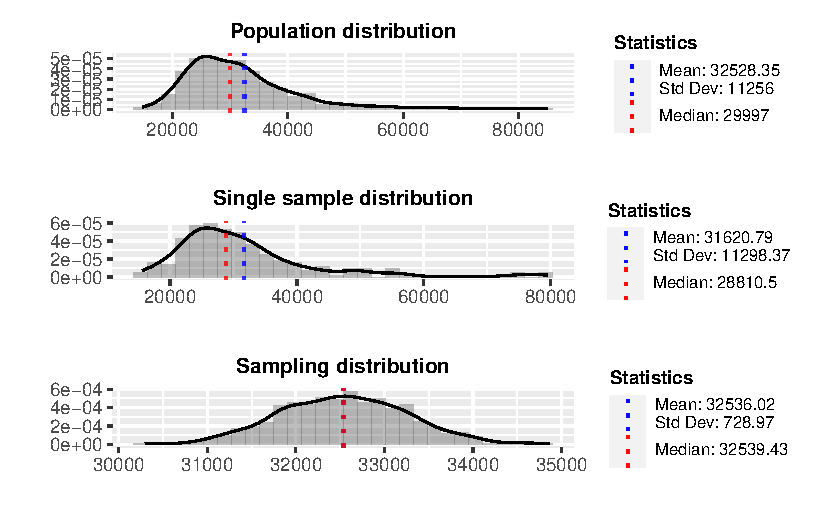
\includegraphics{SSS_5.1-Lecture_files/figure-pdf/unnamed-chunk-7-1.pdf}

\textbf{Usually we cannot know the sampling distribution because we do
not have data on the entire population; we only have data on our single
random sample}

However, hypothesis testing is not based on the true sampling
distribution of the sample mean. It is based on the sampling
distribution under the assumption that the null hypothesis is correct

\begin{itemize}
\tightlist
\item
  Thanks to the central limit theorem, we have a pretty good idea of the
  sampling distribution assuming \(H_0\) is true, even when we only have
  a single random sample!
\end{itemize}

Here we visually stack the following for the variable
\texttt{coa\_grad\_res}:

\begin{itemize}
\tightlist
\item
  the population distribution; distribution from a single random sample;
  and sampling distribution of assuming that \(H_0\) is true
\end{itemize}

\begin{Shaded}
\begin{Highlighting}[]
\FunctionTok{plot\_distribution}\NormalTok{(df\_ipeds\_pop}\SpecialCharTok{$}\NormalTok{coa\_grad\_res, }\AttributeTok{plot\_title =} \StringTok{\textquotesingle{}Population distribution\textquotesingle{}}\NormalTok{) }\SpecialCharTok{+}
  \FunctionTok{plot\_distribution}\NormalTok{(df\_ipeds\_sample}\SpecialCharTok{$}\NormalTok{coa\_grad\_res, }\AttributeTok{plot\_title =} \StringTok{\textquotesingle{}Single sample distribution\textquotesingle{}}\NormalTok{) }\SpecialCharTok{+}
  \FunctionTok{plot\_t\_distribution}\NormalTok{(df\_ipeds\_sample}\SpecialCharTok{$}\NormalTok{coa\_grad\_res, }\AttributeTok{mu =} \DecValTok{28000}\NormalTok{,}\AttributeTok{shade\_rejection =}\NormalTok{ F, }\AttributeTok{shade\_pval =}\NormalTok{ T, }\AttributeTok{plot\_title =} \StringTok{\textquotesingle{}Sampling distribution, assuming H\_0\textquotesingle{}}\NormalTok{) }\SpecialCharTok{+}
  \FunctionTok{plot\_layout}\NormalTok{(}\AttributeTok{ncol =} \DecValTok{1}\NormalTok{)}
\end{Highlighting}
\end{Shaded}

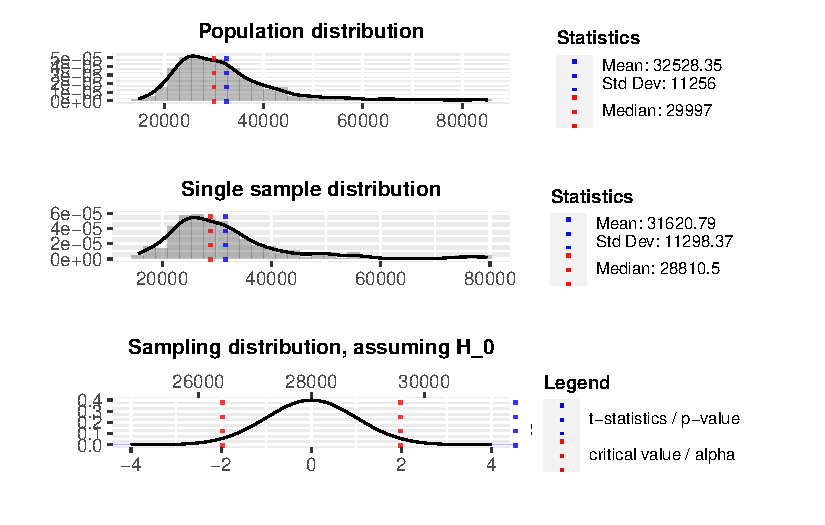
\includegraphics{SSS_5.1-Lecture_files/figure-pdf/unnamed-chunk-8-1.pdf}

The t-test statistic is the distance between the hypothesized \(H_0\)
value and the observed sample estimate value \(\bar{Y}\) scaled in terms
of standard errors

\begin{itemize}
\tightlist
\item
  e.g., it would be unlikely to observe a t-value of greater than
  \texttt{2} or a t-value less than \texttt{-2} because we know (from
  empirical rule and central limit theorem) that 95\% of observations
  fall within two standard deviations of the mean for a normally
  distributed variable
\end{itemize}

\subsection{p-value}\label{p-value}

``p-value'' refers to the probability-value associated with the t-value
from your test statistic

Definition

\begin{itemize}
\tightlist
\item
  Under the assumption that \(H_0\) is true, the \textbf{p-value} is the
  probability of observing a sample estimate (and its associated
  test-statistic) that is at least as far away from the null hypothesis
  value \(\mu_{Y0}\) as the one we observed
\end{itemize}

A small p-value means that it would be unusual to find the sample
estimate we observed if the null hypothesis \(H_0\) is find the observed
data if 𝐻0were true.

Calculating p-value For a two-sided alternative hypothesis
(\(H_a: \mu_Y \neq \mu_{Y0}\))

\begin{itemize}
\tightlist
\item
  let \(t\) be the value of your t-test
\item
  let \(p\) by the p-value associated with \(t\)
\item
  let \(Pr(obs>t)\) is the probability of an observation having a higher
  value of \(t\) than the one you observed
\item
  \(p = Pr(obs > t) + Pr(obs< -t)\)
\item
  Because the sampling distribution is symmetric (because it is normally
  distributed):

  \begin{itemize}
  \tightlist
  \item
    \(Pr(obs >t) = Pr(obs < - t)\)
  \end{itemize}
\item
  therefore, for a two-sided alternative hypothesis

  \begin{itemize}
  \tightlist
  \item
    \(p = 2*Pr(obs > t)\)
  \end{itemize}
\end{itemize}

Let's calculate and visualize p-value for a couple different
hypothesized values of the population mean \(\mu_{Y0}\) for the variable
\texttt{coa\_grad\_res} (full-time, resident grad school cost of
attendance) from the data frame \texttt{df\_ipeds\_sample}

\(H_0: \mu_Y = \mu_{Y0} = \$29,000\) and \(H_a: \mu_Y \neq \$29,000\)

\begin{itemize}
\tightlist
\item
  Sample mean, \(\bar{Y} =\) \ensuremath{3.1620795\times 10^{4}}
\item
  \(t =\) 3.28
\item
  p-value \(= Pr(obs > t) + Pr(obs< -t) =\) 0.001

  \begin{itemize}
  \tightlist
  \item
    \(Pr(obs>t)=\) \ensuremath{6\times 10^{-4}}
  \item
    \(Pr(obs<-t)=\) \ensuremath{6\times 10^{-4}}
  \end{itemize}
\item
  below code chunk runs t-test and plots t-value against sampling
  distribution assuming \(H_0\) is true
\end{itemize}

\begin{Shaded}
\begin{Highlighting}[]
\FunctionTok{mean}\NormalTok{(}\AttributeTok{x =}\NormalTok{ df\_ipeds\_sample}\SpecialCharTok{$}\NormalTok{coa\_grad\_res)}
\CommentTok{\#\textgreater{} [1] 31620.8}
\FunctionTok{t.test}\NormalTok{(}\AttributeTok{x =}\NormalTok{ df\_ipeds\_sample}\SpecialCharTok{$}\NormalTok{coa\_grad\_res, }\AttributeTok{mu =} \DecValTok{29000}\NormalTok{)}
\CommentTok{\#\textgreater{} }
\CommentTok{\#\textgreater{}  One Sample t{-}test}
\CommentTok{\#\textgreater{} }
\CommentTok{\#\textgreater{} data:  df\_ipeds\_sample$coa\_grad\_res}
\CommentTok{\#\textgreater{} t = 3.2804, df = 199, p{-}value = 0.001224}
\CommentTok{\#\textgreater{} alternative hypothesis: true mean is not equal to 29000}
\CommentTok{\#\textgreater{} 95 percent confidence interval:}
\CommentTok{\#\textgreater{}  30045.37 33196.22}
\CommentTok{\#\textgreater{} sample estimates:}
\CommentTok{\#\textgreater{} mean of x }
\CommentTok{\#\textgreater{}   31620.8}
\FunctionTok{plot\_t\_distribution}\NormalTok{(df\_ipeds\_sample}\SpecialCharTok{$}\NormalTok{coa\_grad\_res, }\AttributeTok{mu =} \DecValTok{29000}\NormalTok{,}\AttributeTok{shade\_rejection =}\NormalTok{ F, }\AttributeTok{shade\_pval =}\NormalTok{ T)}
\end{Highlighting}
\end{Shaded}

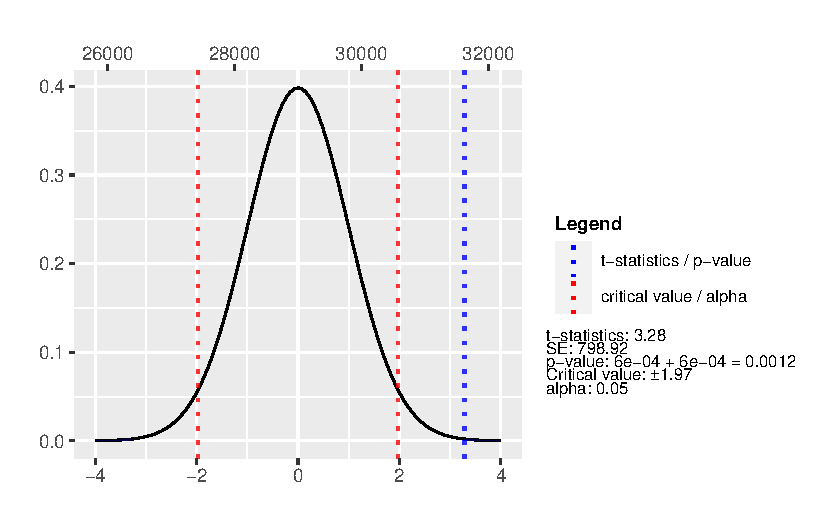
\includegraphics{SSS_5.1-Lecture_files/figure-pdf/unnamed-chunk-9-1.pdf}

\(H_0: \mu_Y = \mu_{Y0} = \$28,000\) and \(H_a: \mu_Y \ne \$28,000\)

\begin{itemize}
\tightlist
\item
  Sample mean, \$\bar\{Y\} = \$ \ensuremath{3.1620795\times 10^{4}}
\item
  \(t =\) 4.53
\item
  p-value \(= Pr(obs > t) + Pr(obs< -t) =\) 0

  \begin{itemize}
  \tightlist
  \item
    \(Pr(obs>t)=\) 0
  \item
    \(Pr(obs<-t)=\) 0
  \end{itemize}
\item
  below code chunk runs t-test and plots t-value against sampling
  distribution assuming \(H_0\) is true
\end{itemize}

\begin{Shaded}
\begin{Highlighting}[]
\FunctionTok{mean}\NormalTok{(}\AttributeTok{x =}\NormalTok{ df\_ipeds\_sample}\SpecialCharTok{$}\NormalTok{coa\_grad\_res)}
\CommentTok{\#\textgreater{} [1] 31620.8}
\FunctionTok{t.test}\NormalTok{(}\AttributeTok{x =}\NormalTok{ df\_ipeds\_sample}\SpecialCharTok{$}\NormalTok{coa\_grad\_res, }\AttributeTok{mu =} \DecValTok{28000}\NormalTok{)}
\CommentTok{\#\textgreater{} }
\CommentTok{\#\textgreater{}  One Sample t{-}test}
\CommentTok{\#\textgreater{} }
\CommentTok{\#\textgreater{} data:  df\_ipeds\_sample$coa\_grad\_res}
\CommentTok{\#\textgreater{} t = 4.5321, df = 199, p{-}value = 1.006e{-}05}
\CommentTok{\#\textgreater{} alternative hypothesis: true mean is not equal to 28000}
\CommentTok{\#\textgreater{} 95 percent confidence interval:}
\CommentTok{\#\textgreater{}  30045.37 33196.22}
\CommentTok{\#\textgreater{} sample estimates:}
\CommentTok{\#\textgreater{} mean of x }
\CommentTok{\#\textgreater{}   31620.8}
\FunctionTok{plot\_t\_distribution}\NormalTok{(df\_ipeds\_sample}\SpecialCharTok{$}\NormalTok{coa\_grad\_res, }\AttributeTok{mu =} \DecValTok{28000}\NormalTok{,}\AttributeTok{shade\_rejection =}\NormalTok{ F, }\AttributeTok{shade\_pval =}\NormalTok{ T)}
\end{Highlighting}
\end{Shaded}

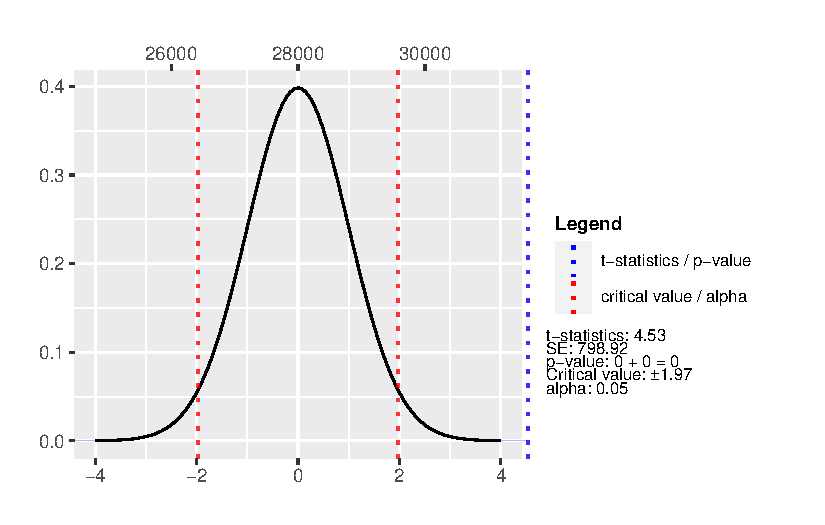
\includegraphics{SSS_5.1-Lecture_files/figure-pdf/unnamed-chunk-10-1.pdf}

\(H_0: \mu_Y = \mu_{Y0} = \$31,500\) and \(H_a: \mu_Y \neq \$31,500\)

\begin{itemize}
\tightlist
\item
  Sample mean, \(\bar{Y} =\) \ensuremath{3.1620795\times 10^{4}}
\item
  \(t =\) 0.15
\item
  p-value \(= Pr(obs > t) + Pr(obs< -t) =\) 0.88

  \begin{itemize}
  \tightlist
  \item
    \(Pr(obs>t)=\) 0.44
  \item
    \(Pr(obs<-t)=\) 0.44
  \end{itemize}
\item
  below code chunk runs t-test and plots t-value against sampling
  distribution assuming \(H_0\) is true
\end{itemize}

\begin{Shaded}
\begin{Highlighting}[]
\FunctionTok{mean}\NormalTok{(}\AttributeTok{x =}\NormalTok{ df\_ipeds\_sample}\SpecialCharTok{$}\NormalTok{coa\_grad\_res)}
\CommentTok{\#\textgreater{} [1] 31620.8}
\FunctionTok{t.test}\NormalTok{(}\AttributeTok{x =}\NormalTok{ df\_ipeds\_sample}\SpecialCharTok{$}\NormalTok{coa\_grad\_res, }\AttributeTok{mu =} \DecValTok{31500}\NormalTok{)}
\CommentTok{\#\textgreater{} }
\CommentTok{\#\textgreater{}  One Sample t{-}test}
\CommentTok{\#\textgreater{} }
\CommentTok{\#\textgreater{} data:  df\_ipeds\_sample$coa\_grad\_res}
\CommentTok{\#\textgreater{} t = 0.1512, df = 199, p{-}value = 0.88}
\CommentTok{\#\textgreater{} alternative hypothesis: true mean is not equal to 31500}
\CommentTok{\#\textgreater{} 95 percent confidence interval:}
\CommentTok{\#\textgreater{}  30045.37 33196.22}
\CommentTok{\#\textgreater{} sample estimates:}
\CommentTok{\#\textgreater{} mean of x }
\CommentTok{\#\textgreater{}   31620.8}
\FunctionTok{plot\_t\_distribution}\NormalTok{(df\_ipeds\_sample}\SpecialCharTok{$}\NormalTok{coa\_grad\_res, }\AttributeTok{mu =} \DecValTok{31500}\NormalTok{)}
\end{Highlighting}
\end{Shaded}

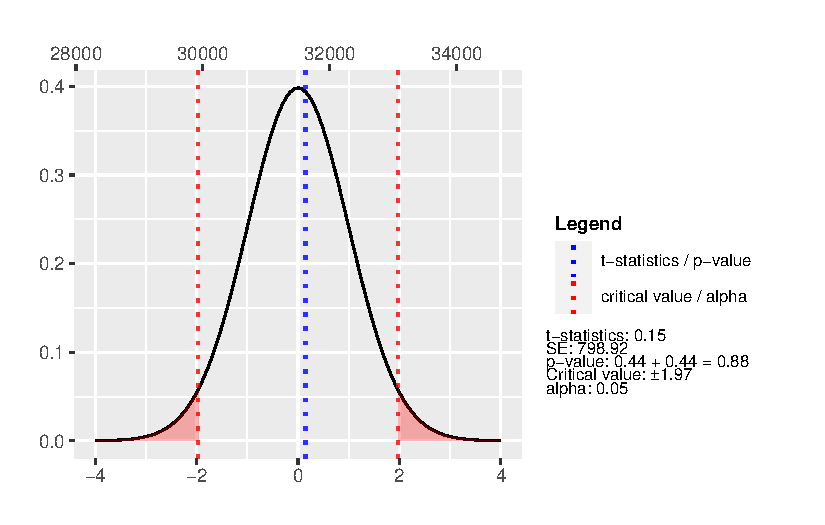
\includegraphics{SSS_5.1-Lecture_files/figure-pdf/unnamed-chunk-11-1.pdf}

\subsection{Rejection region and
conclusion}\label{rejection-region-and-conclusion}

\subsubsection{Alpha level (rejection
region)}\label{alpha-level-rejection-region}

\(\alpha\) level (referred to as ``alpha level'' or ``rejection
region'')

\begin{itemize}
\tightlist
\item
  Definition: \(\alpha\) level is a number such that we reject the null
  hypothesis \(H_0\) the observed p-value is less than or equal to the
  alpha level.
\end{itemize}

In practice, the most common alpha level \(\alpha\) is \texttt{.05}

\begin{itemize}
\tightlist
\item
  e.g., if we choose \(\alpha= .05\) and our t-statistic is associated
  with a p-value of .02, then we reject \(H_0\); if we choose
  \(\alpha= .05\) and our t-statistic is associated with a p-value of
  .07, then we do not reject \(H_0\)
\item
  sometimes researchers choose an alpha level of \texttt{.10} but
  usually this is viewed as not sufficiently strong threshold to reject
  \(H_0\)
\end{itemize}

Usually, you define alpha level \textbf{prior} to running analyses

\begin{itemize}
\tightlist
\item
  when researchers define alpha level (rejection region) \emph{after}
  running analyses, there may be a temptation to choose an alpha level
  that allows them to reject \(H_0\)
\end{itemize}

To show how alpha level is used in practice, we'll test the null
hypothesis that population mean grad resident cost of attendance is
\texttt{28,500}, initially using an alpha level of .05

\begin{itemize}
\tightlist
\item
  \(H_0: \mu_Y = \mu_{Y0} = \$28,500\) and \(H_a: \mu_Y \neq \$28,500\)
\item
  Sample mean, \(\bar{Y} =\) \ensuremath{3.1620795\times 10^{4}}
\item
  \(t =\) 3.91
\item
  p-value \(= Pr(obs > t) + Pr(obs< -t) =\) 0

  \begin{itemize}
  \tightlist
  \item
    \(Pr(obs>t)=\) \ensuremath{10^{-4}}
  \item
    \(Pr(obs<-t)=\) \ensuremath{10^{-4}}
  \end{itemize}
\end{itemize}

Note that the \texttt{t.test()} function doesn't have an argument that
let's you specify the alpha level (rejection region); rather, the idea
is that you choose the alpha level and then compare that to the p-value
calculated by \texttt{t.test()}

\begin{Shaded}
\begin{Highlighting}[]
\FunctionTok{t.test}\NormalTok{(}\AttributeTok{x =}\NormalTok{ df\_ipeds\_sample}\SpecialCharTok{$}\NormalTok{coa\_grad\_res, }\AttributeTok{mu =} \DecValTok{28500}\NormalTok{)}
\CommentTok{\#\textgreater{} }
\CommentTok{\#\textgreater{}  One Sample t{-}test}
\CommentTok{\#\textgreater{} }
\CommentTok{\#\textgreater{} data:  df\_ipeds\_sample$coa\_grad\_res}
\CommentTok{\#\textgreater{} t = 3.9063, df = 199, p{-}value = 0.0001284}
\CommentTok{\#\textgreater{} alternative hypothesis: true mean is not equal to 28500}
\CommentTok{\#\textgreater{} 95 percent confidence interval:}
\CommentTok{\#\textgreater{}  30045.37 33196.22}
\CommentTok{\#\textgreater{} sample estimates:}
\CommentTok{\#\textgreater{} mean of x }
\CommentTok{\#\textgreater{}   31620.8}
\end{Highlighting}
\end{Shaded}

Note that the user-defined \texttt{plot\_t\_distribution()} includes an
optional argument that allows you to specify the alpha-level

\begin{itemize}
\tightlist
\item
  syntax (including default argument values for arguments with defaults)

  \begin{itemize}
  \tightlist
  \item
    \texttt{plot\_t\_distribution(data\_vec,\ mu,\ alpha\ =\ 0.05,\ alternative\ =\ \textquotesingle{}two.sided\textquotesingle{},\ plot\_title\ =\ \textquotesingle{}\textquotesingle{})}
  \item
    So we can set the alpha level with the argument \texttt{alpha},
    which has the default value of \texttt{0.05}
  \end{itemize}
\end{itemize}

Below, we run \texttt{plot\_t\_distribution()}, manually setting the
\texttt{alpha} argument to the the default value of \texttt{0.05}

\begin{itemize}
\tightlist
\item
  the blue dotted line denotes the t-value from our test statistic

  \begin{itemize}
  \tightlist
  \item
    \(t =\) 3.91
  \end{itemize}
\item
  the red dotted lines denote the t-value associated with the chosen
  alpha level (rejection region)

  \begin{itemize}
  \tightlist
  \item
    the t-value associated with the alpha level is referred to as the
    ``critical value''
  \item
    the t-statistic of 3.91 is less than the critical value of 1.97,
    indicating that we won't reject \(H_0\)
  \end{itemize}
\item
  the shaded region denotes the probability associated with the chosen
  alpha level

  \begin{itemize}
  \tightlist
  \item
    given our choice of \texttt{alpha\ =\ .05}, the shaded region
    represents .05, that is the percent of all observations that lie in
    the rejection region
  \item
    our p-value of 0.001 is greater than our alpha level of .05,
    indicating that we won't reject \(H_0\)
  \end{itemize}
\item
  Since our p-value is greater than our alpha level, we do not reject
  \(H_0\)
\end{itemize}

\begin{Shaded}
\begin{Highlighting}[]
\FunctionTok{plot\_t\_distribution}\NormalTok{(df\_ipeds\_sample}\SpecialCharTok{$}\NormalTok{coa\_grad\_res, }\AttributeTok{mu =} \DecValTok{28500}\NormalTok{, }\AttributeTok{alpha =}\NormalTok{ .}\DecValTok{05}\NormalTok{)}
\end{Highlighting}
\end{Shaded}

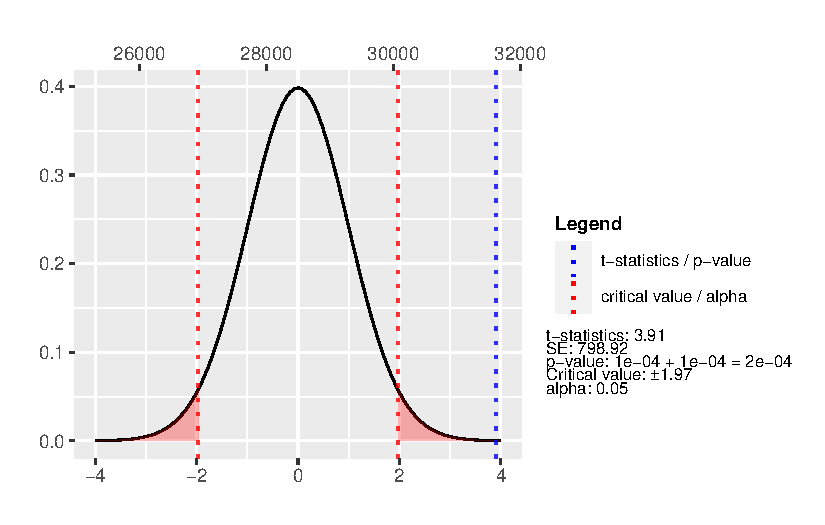
\includegraphics{SSS_5.1-Lecture_files/figure-pdf/unnamed-chunk-13-1.pdf}

How would our conclusion change if we chose an alpha level of .10?

\begin{itemize}
\tightlist
\item
  \(H_0: \mu_Y = \mu_{Y0} = \$28,500\) and \(H_a: \mu_Y \ne \$28,500\)
\item
  Sample mean, \(\bar{Y} =\) \ensuremath{3.1620795\times 10^{4}}
\item
  \(t =\) 3.91
\item
  p-value \(= Pr(obs > t) + Pr(obs< -t) =\) 0

  \begin{itemize}
  \tightlist
  \item
    \(Pr(obs>t)=\) \ensuremath{10^{-4}}
  \item
    \(Pr(obs<-t)=\) \ensuremath{10^{-4}}
  \end{itemize}
\item
  Since our p-value of 0 is less than the alpha level of .10, we reject
  \(H_0\)
\end{itemize}

\begin{Shaded}
\begin{Highlighting}[]
\FunctionTok{plot\_t\_distribution}\NormalTok{(df\_ipeds\_sample}\SpecialCharTok{$}\NormalTok{coa\_grad\_res, }\AttributeTok{mu =} \DecValTok{28500}\NormalTok{, }\AttributeTok{alpha =}\NormalTok{ .}\DecValTok{10}\NormalTok{)}
\end{Highlighting}
\end{Shaded}

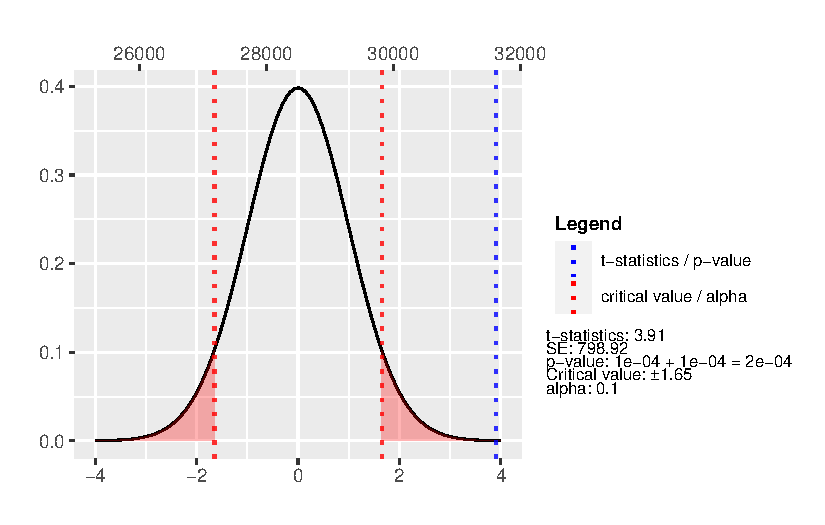
\includegraphics{SSS_5.1-Lecture_files/figure-pdf/unnamed-chunk-14-1.pdf}

\subsubsection{Conclusion}\label{conclusion}

Last step is to make a conclusion about your hypothesis based on
comparing the p-value you observed to the alpha level

\textbf{How to state the conclusion}

\begin{itemize}
\tightlist
\item
  if p-value is greater than the alpha level \(\alpha\) (e.g.,
  \(p-val =.06, \alpha = .05\))

  \begin{itemize}
  \tightlist
  \item
    conclusion: do not reject \(H_0\)
  \item
    longer version: ``We do not have sufficient evidence to reject the
    null hypothesis, \(H_0\), that population mean \(\mu_Y\) is equal to
    \(\mu_{Y0}\)''
  \item
    do not say ``we accept \(H_0\) because we don't know the exact value
    of the population parameter
  \end{itemize}
\item
  if p-value is less than the alpha level \(\alpha\) (e.g.,
  \(p-val =.04, \alpha = .05\))

  \begin{itemize}
  \tightlist
  \item
    conclusion: we reject \(H_0\)

    \begin{itemize}
    \tightlist
    \item
      can also say ``we accept \(H_a\), but people usually say''reject
      \(H_0\)
    \end{itemize}
  \item
    longer version: ``we reject the null hypothesis \(H_0\), that
    population mean \(\mu_Y\) is equal to \(\mu_{Y0}\)''
  \end{itemize}
\end{itemize}

This example:

\begin{itemize}
\tightlist
\item
  \(H_0: \mu_Y = \mu_{Y0} = \$28,500\) and \(H_a: \mu_Y \ne \$28,500\)
  and alpha level \(\alpha = .05\)
\item
  p-value \(= Pr(obs > t) + Pr(obs< -t) =\) 0
\item
  conclusion:

  \begin{itemize}
  \tightlist
  \item
    do not reject \(H_0\)
  \item
    We do not have sufficient evidence to reject the null hypothesis,
    \(H_0\), that population mean full-time resident graduate cost of
    attendance is equal to \texttt{28,500}
  \end{itemize}
\end{itemize}

\begin{Shaded}
\begin{Highlighting}[]
\FunctionTok{plot\_t\_distribution}\NormalTok{(df\_ipeds\_sample}\SpecialCharTok{$}\NormalTok{coa\_grad\_res, }\AttributeTok{mu =} \DecValTok{28500}\NormalTok{, }\AttributeTok{alpha =}\NormalTok{ .}\DecValTok{05}\NormalTok{,}
                    \AttributeTok{shade\_rejection =} \ConstantTok{TRUE}\NormalTok{, }\AttributeTok{shade\_pval =} \ConstantTok{FALSE}\NormalTok{)}
\end{Highlighting}
\end{Shaded}

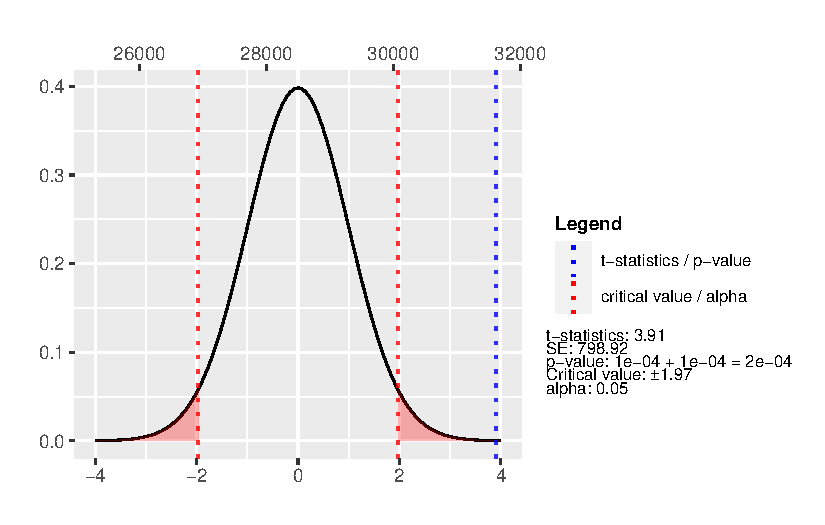
\includegraphics{SSS_5.1-Lecture_files/figure-pdf/unnamed-chunk-15-1.pdf}



\end{document}
